
\documentclass[fleqn,addpoints]{exam}

\usepackage{graphicx}
\usepackage{booktabs}
\usepackage{float}
\usepackage{amsmath}
\usepackage{cancel}
\usepackage{polynom}
\usepackage{caption}
\usepackage{mdwlist}

\newcommand{\degree}{\ensuremath{^\circ}} 

\printanswers

\ifprintanswers 
\usepackage{2in1, lscape} 
\fi

\title{Math 115 \\ Homework 20}
\date{April 26, 2011}

\begin{document}

\maketitle

% \begin{figure}[H]
%   \centering
%   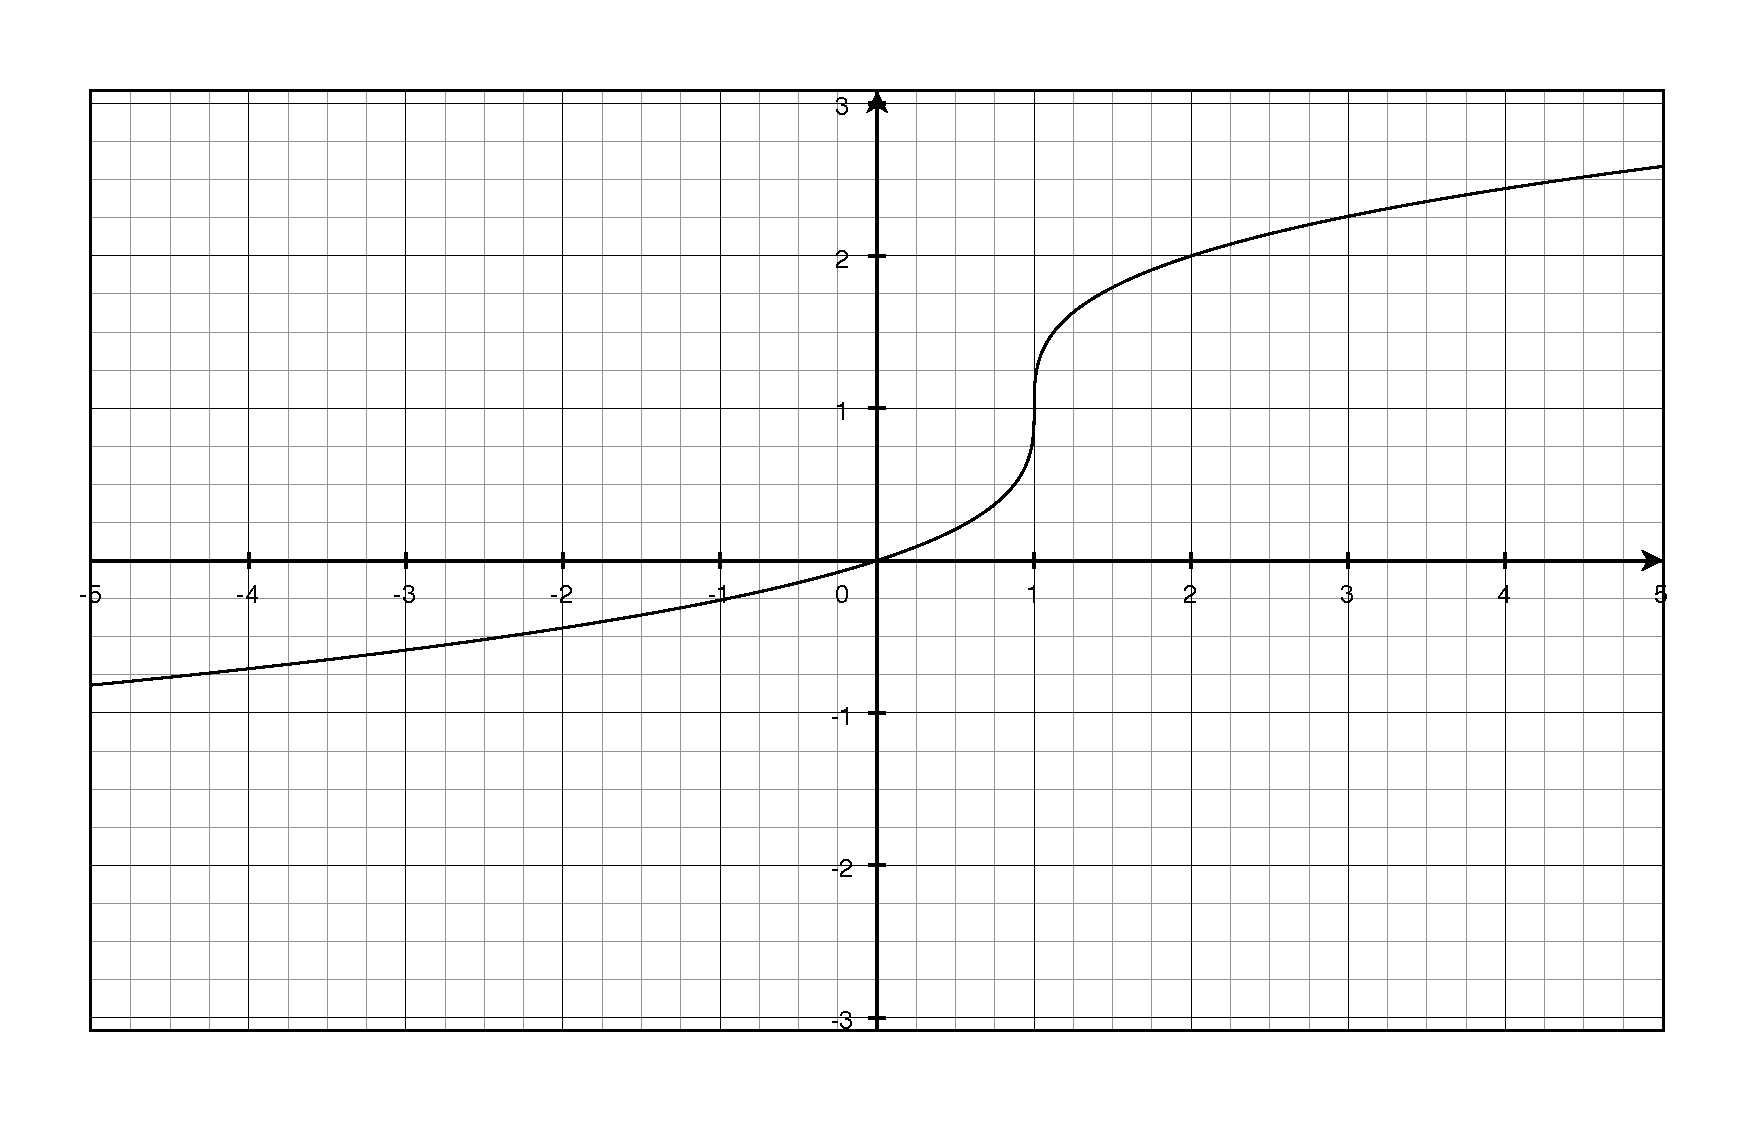
\includegraphics[scale=.3]{question7.eps}
%   \caption*{Question 7}
% \end{figure}

\section{Homework}
\begin{itemize}
  \item pp 359-362: 7-8, 13-14, 21-22, 25-26, 29-30, 37-38, 41-42, 55-56, 59-60, 67-68, 83-84, 97-98, 103-106
  \item pp 368-369: 1-10, 15-19, 25-26, 29-32, 59-60, 61-62
\end{itemize}

\section{Extra Credit}

\begin{itemize}
\item p. 362, question 102

\begin{solution}
\begin{description}
\item[a]

\begin{itemize*}
\item For each revolution of the pedals, the chain travels the circumference of the front gear or $8 \pi$ inches.  
\item When the chain travels $8 \pi$ inches, the gear on the wheel makes $\dfrac{8 \pi}{2 \cdot 2 \pi} = 2$ revolutions.
\item With one revolution of the wheel, the bike travels $14 \cdot 2 \pi = 28 \pi$ inches.  So the bike is traveling at 
  $28 \pi \cdot 2 = 56 \pi \approx 176$ inches per second.
\end{itemize*}

\item[b]

To convert from inches to miles and seconds to hours, you need to do something like this:
\[
  176 \cdot \frac{1}{12} \cdot \frac{1}{5280} \cdot \frac{60}{1} \cdot \frac{60}{1} \approx 10
\]

So the bike is traveling about 10 mph.

\end{description}

\end{solution}

\item 
Move one digit to make the following equation true (sort of a trick):
\[
  62 - 63 = 1
\] 
\begin{solution}
\[
  2^6 - 63 = 64 - 63 = 1
\] 
\end{solution}

\end{itemize}

\ifprintanswers
\section{Pages 359-362}

\begin{description}
\item[7]
I

\item[8]
% \[
% \pi < \frac{7 \pi}{5} < \frac{3 \pi}{2}
% \]
III

% \item[13]
% \begin{description}
% \item[a]
% \begin{figure}[H]
%   \centering
%   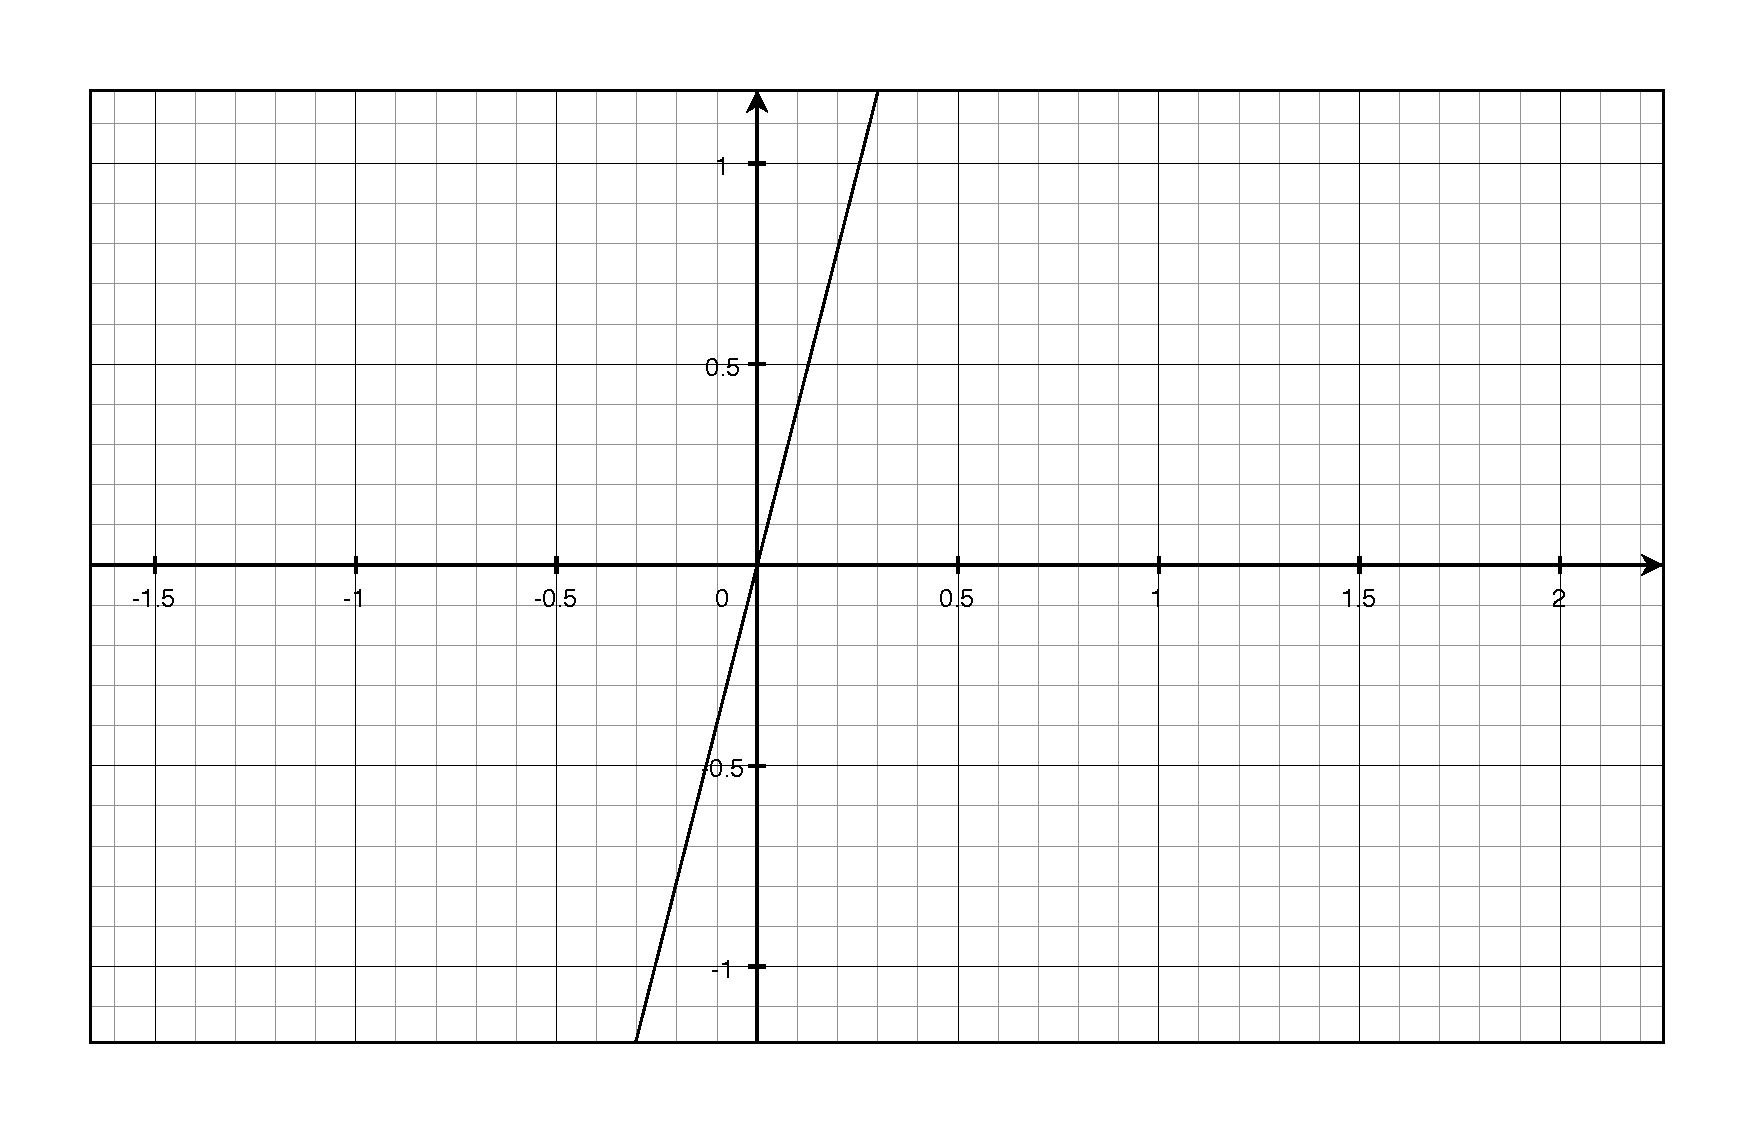
\includegraphics[scale=.3]{question13a.eps}
%   \caption*{13 a}
% \end{figure}

% \item[b]
% \begin{figure}[H]
%   \centering
%   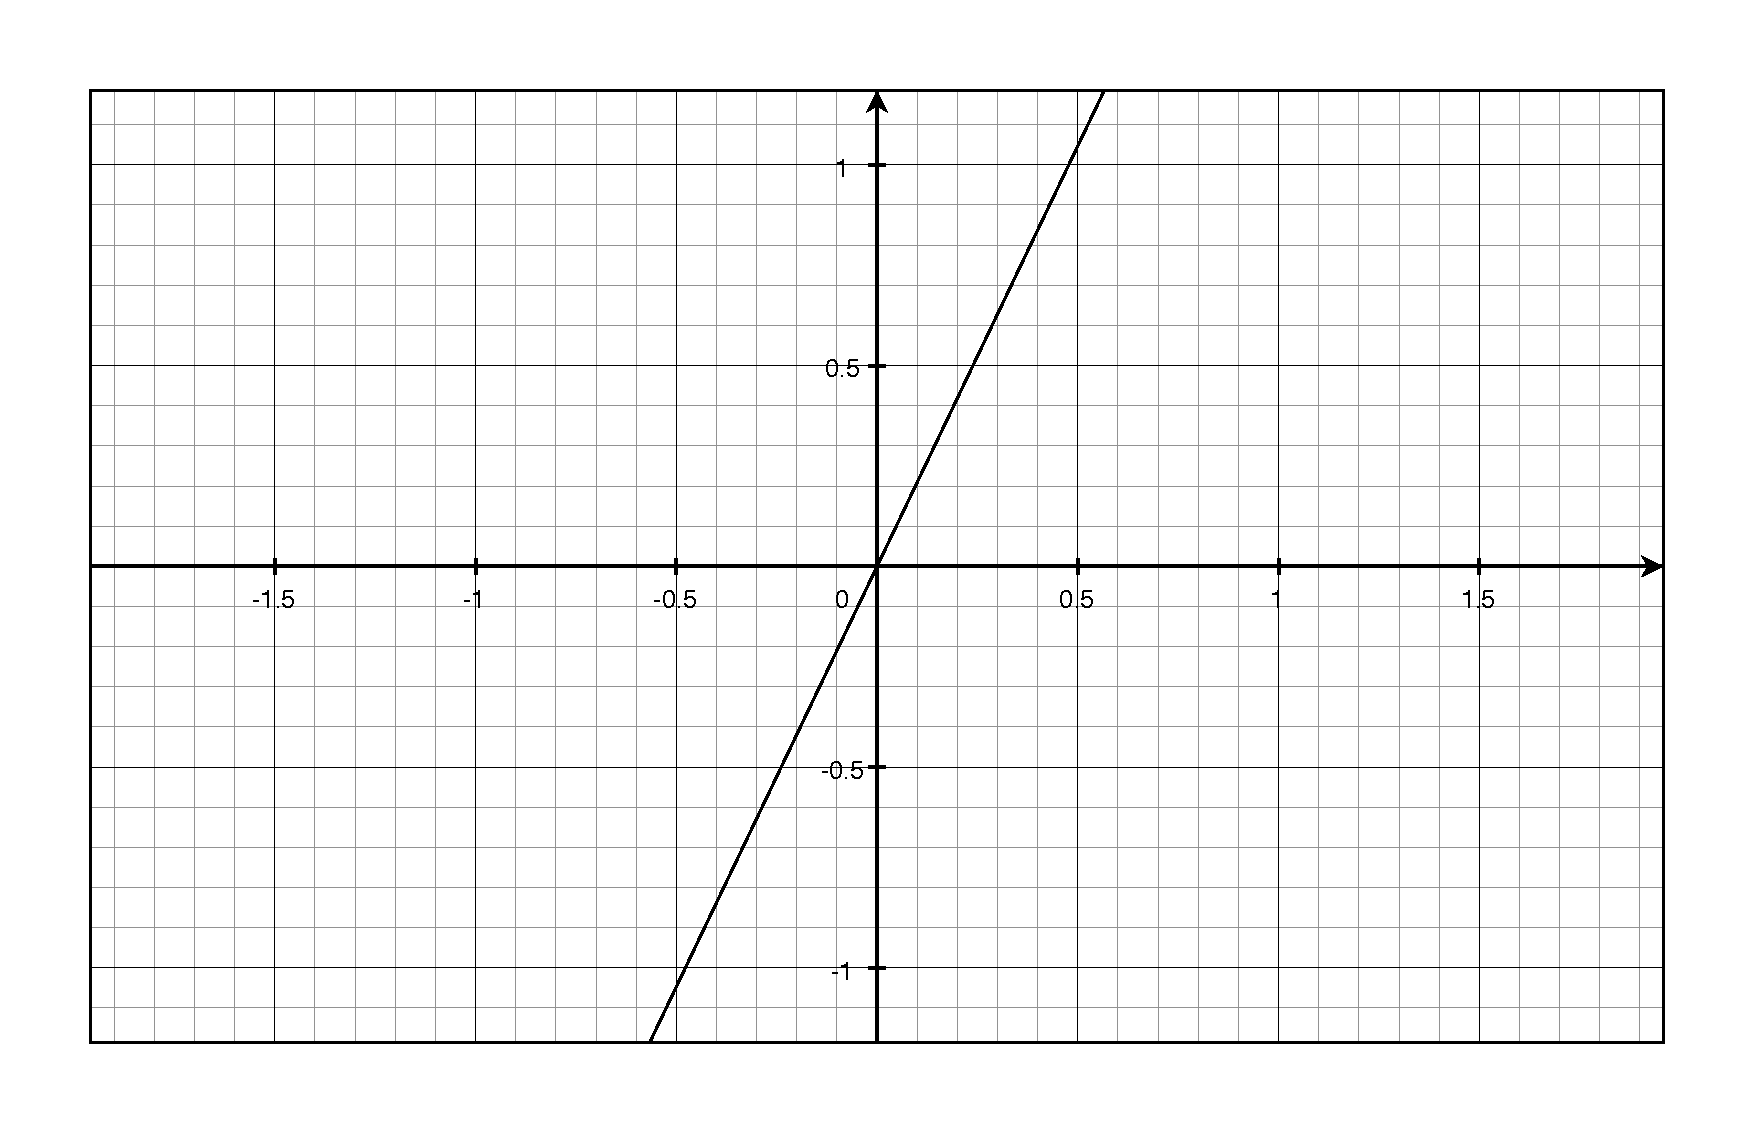
\includegraphics[scale=.3]{question13b.eps}
%   \caption*{13 b}
% \end{figure}

% \end{description}

% \item[14]
% \begin{description}
% \item[a]
% \begin{figure}[H]
%   \centering
%   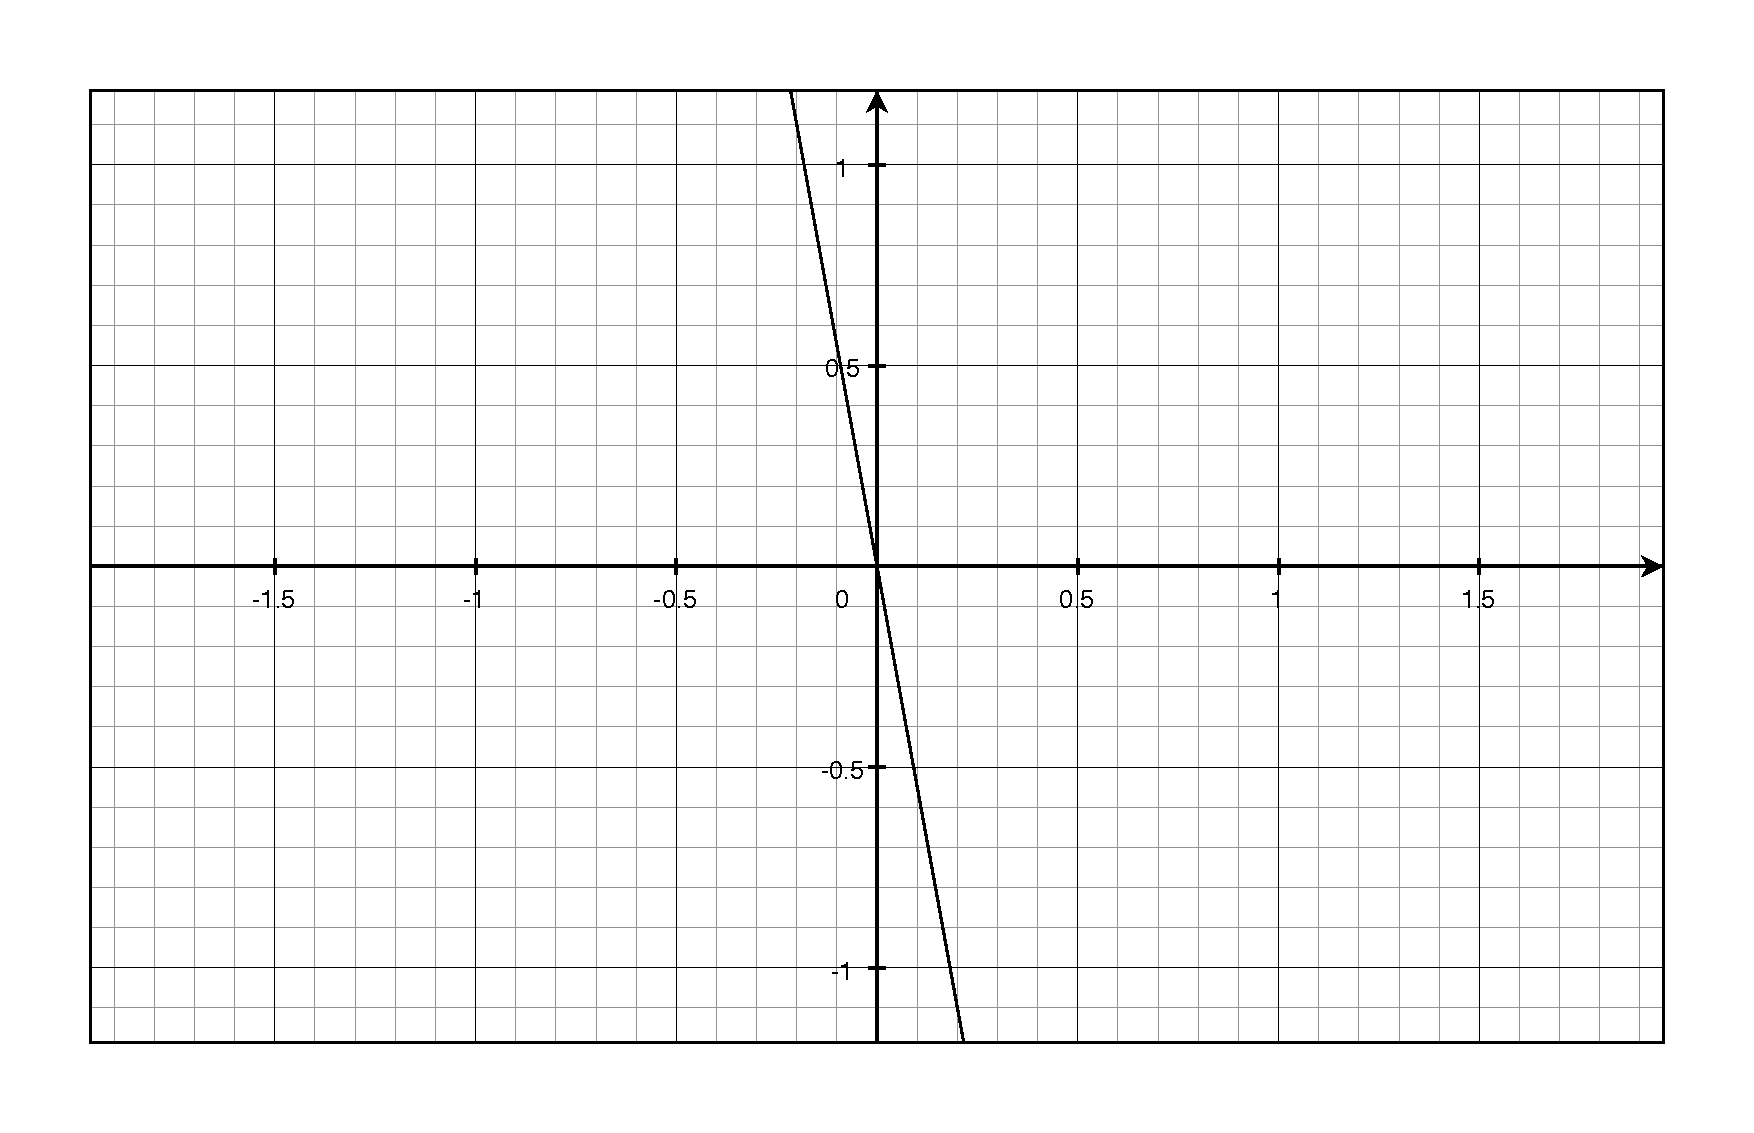
\includegraphics[scale=.3]{question14a.eps}
%   \caption*{14 a}
% \end{figure}

% \item[b]
% \begin{figure}[H]
%   \centering
%   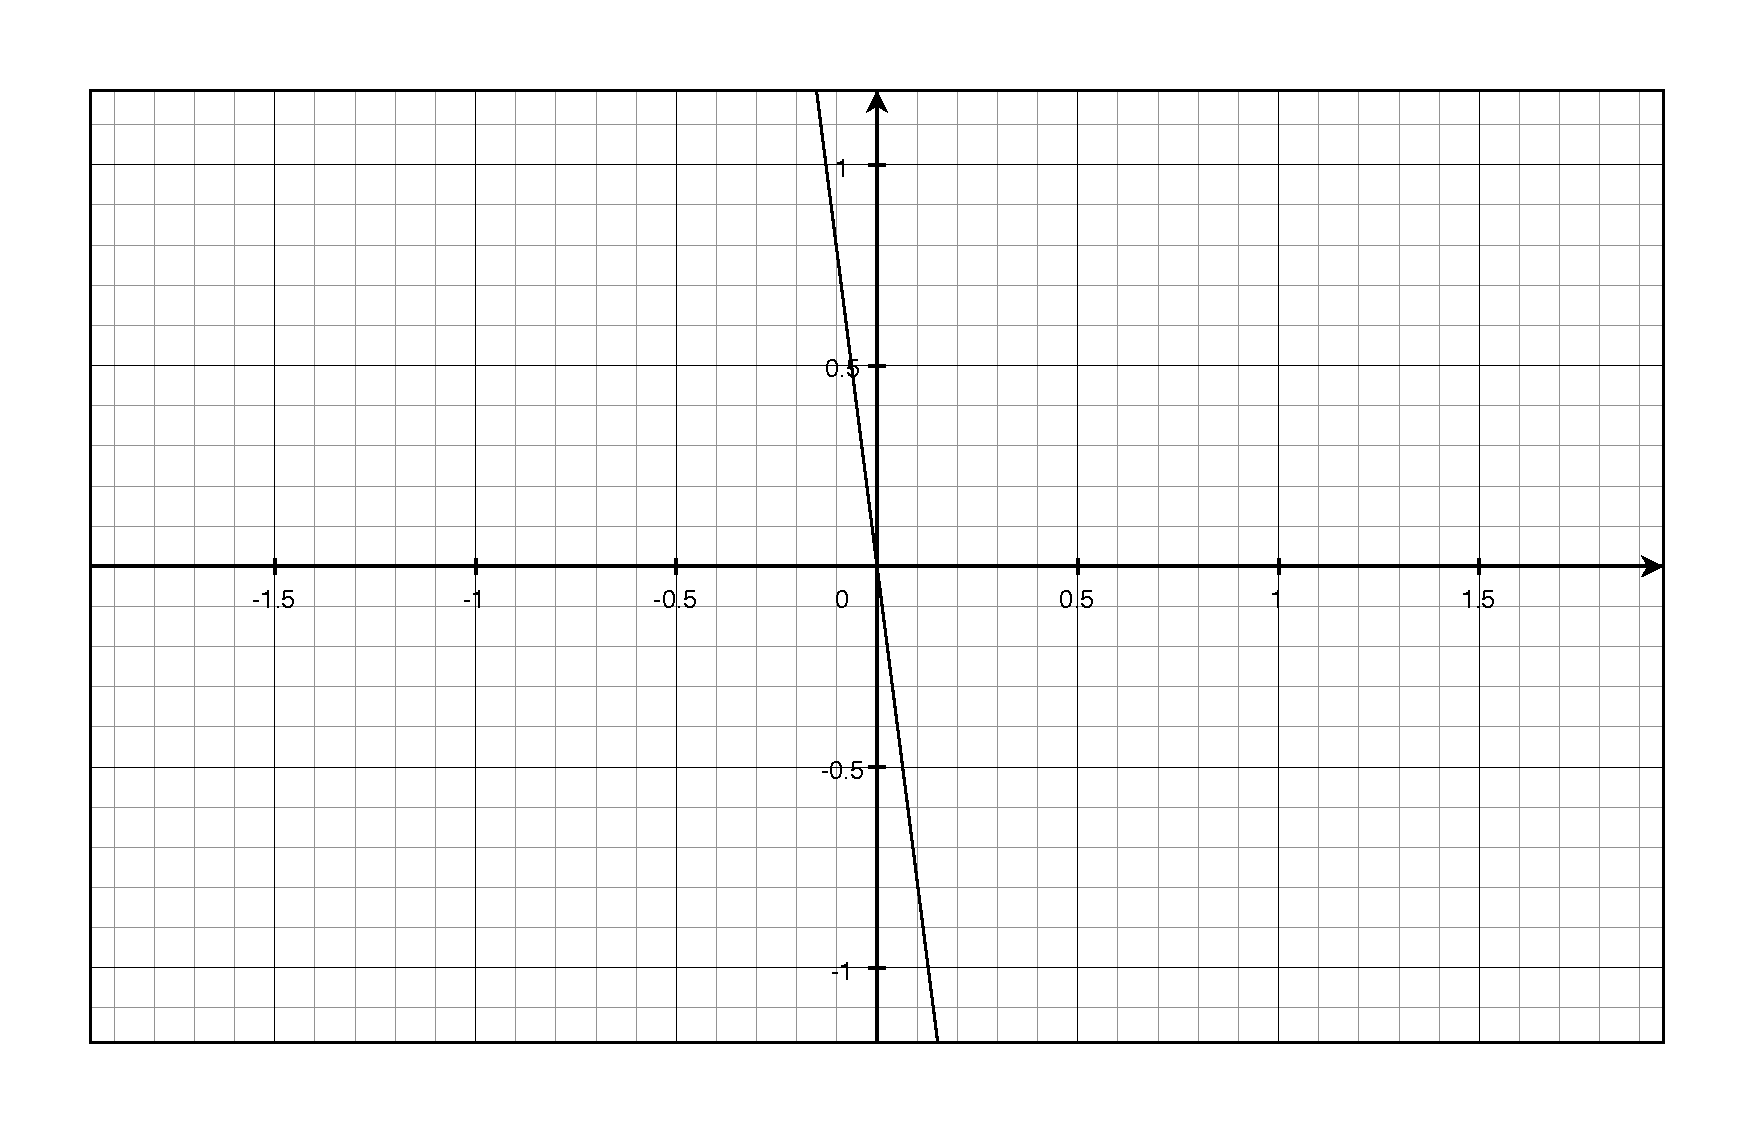
\includegraphics[scale=.3]{question14b.eps}
%   \caption*{14 b}
% \end{figure}

% \end{description}

\item[21]
\begin{description}
\item[a]
complement:
\[
  \frac{\pi}{2} - \frac{\pi}{3} = \frac{\pi}{6}
\]

supplement:
\[
  \pi - \frac{\pi}{3} = \frac{2 \pi}{3}
\]

\item[b]
no complement:

supplement:
\[
  \pi - \frac{3 \pi}{4} = \frac{\pi}{4}
\]


\end{description}

\item[22]
\begin{description}
\item[a]
complement:
\[
  \frac{\pi}{2} - \frac{\pi}{12} = \frac{5 \pi}{12}
\]

supplement:
\[
  \pi - \frac{\pi}{12} = \frac{11 \pi}{12}
\]

\item[b]
no complement:

supplement:
\[
  \pi - \frac{11 \pi}{12} = \frac{\pi}{12}
\]

\end{description}

\item[25]

\begin{description}
\item[a]
\[
  30 \degree = 30\degree \left( \frac{\pi}{180 \degree} \right) = \frac{\pi}{6}
\]

\item[b]
\[
  150 \degree = 150\degree \left( \frac{\pi}{180 \degree} \right) = \frac{5\pi}{6}
\]
\end{description}

\item[26]

\begin{description}
\item[a]
\[
  315 \degree = 315 \degree \left( \frac{\pi}{180\degree} \right) = \frac{7 \pi}{4}
\]

\item[b]
\[
  120 \degree = 120 \degree \left( \frac{\pi}{180\degree} \right) = \frac{2 \pi}{3}
\]
\end{description}

\item[29]
\[
  115 \degree = 115 \degree \left( \frac{\pi}{180\degree} \right) = 2.007
\]

\item[30]
\[
  87.4 \degree = 87.4 \degree \left( \frac{\pi}{180\degree} \right) = 1.525
\]

\item[37]

\begin{description}
\item[a]
\[
  \frac{3 \pi}{2} = \frac{3 \pi}{2} \cdot \frac{180 \degree}{\pi} = 270 \degree
\]

\item[b]
\[
  \frac{7 \pi}{6} = \frac{7 \pi}{6} \cdot \frac{180 \degree}{\pi} = 210 \degree
\]
\end{description}

\item[38]

\begin{description}
\item[a]
\[
  - \frac{7 \pi}{12} = - \frac{7 \pi}{12} \cdot \frac{180 \degree}{\pi} = -105 \degree
\]

\item[b]
\[
  \frac{\pi}{9} = \frac{\pi}{9} \cdot \frac{180 \degree}{\pi} = 20 \degree
\]
\end{description}

\item[41]
\[
  \frac{\pi}{7} = \frac{\pi}{7} \cdot \frac{180 \degree}{\pi} = 25.714 \degree
\]

\item[42]
\[
  \frac{5 \pi}{11} = \frac{5 \pi}{11} \cdot \frac{180 \degree}{\pi} = 81.818 \degree
\]

\item[55]
\begin{description}
\item[a] II
\item[b] IV
\end{description}

\item[56]
\begin{description}
\item[a] I
\item[b] III
\end{description}

\item[67]
\begin{description}
\item[a] 
\begin{itemize*}
\item complement: $90\degree - 18\degree = 72\degree$
\item supplement: $180\degree - 18\degree = 162\degree$
\end{itemize*}

\item[b] 
\begin{itemize*}
\item no complement
\item supplement: $180\degree - 115\degree = 65\degree$
\end{itemize*}

\end{description}

\item[68]
\begin{description}
\item[a] 
\begin{itemize*}
\item complement: $90\degree - 3\degree = 87\degree$
\item supplement: $180\degree - 3\degree = 177\degree$
\end{itemize*}

\item[b] 
\begin{itemize*}
\item complement: $90\degree - 64\degree = 26\degree$
\item supplement: $180\degree - 64\degree = 116\degree$
\end{itemize*}

\end{description}

\item[83]
\[
  \frac{6}{27} = \frac{2}{9} \approx 0.222
\]

\item[84]
\[
  \frac{14}{8} = \frac{7}{4} = 1.75 
\]

\item[97]
\[
  \frac{2.5}{6} = \frac{5}{12} \approx 0.417 
\]

\item[98]
The radius of the hoist is 5 inches, so the required angle in radians is $\dfrac{24}{5}$

To convert to degrees:
\[
  \frac{24}{5} \cdot \frac{180}{\pi} = 275 \degree
\]

\item[103]
false.  $4 \pi$ radians is two complete revolutions

\item[104]
true

\item[105]
\begin{description}
\item[a] an angle with the initial side on the positive x-axis and the vertex at the origin
\item[b] an angle measured in the clockwise direction
\item[c] angles in standard position with the same terminal side
\item[d] an angle between $\dfrac{\pi}{2}$ and $\pi$ radians
\end{description}

\item[106]
With a larger diameter fan the tips have farther to go in the same time so they move faster
\end{description}

\section{Pages 368-369}
\begin{description}
\item[1]

\begin{tabular}{cccccc}
\toprule
sin & cos & tan & csc & sec & cot \\
\midrule
  $\dfrac{15}{17}$ &  $-\dfrac{8}{17}$ & $-\dfrac{15}{8}$ & $\dfrac{17}{15}$ & $-\dfrac{17}{8}$ & $-\dfrac{8}{15}$ \\
\bottomrule
\end{tabular}

\item[2]
\begin{tabular}{cccccc}
\toprule
sin & cos & tan & csc & sec & cot \\
\midrule
  $\dfrac{5}{13}$ &  $\dfrac{12}{13}$ & $\dfrac{5}{12}$ & $\dfrac{13}{5}$ & $\dfrac{13}{12}$ & $\dfrac{12}{5}$ \\
\bottomrule
\end{tabular}

\item[3]
\begin{tabular}{cccccc}
\toprule
sin & cos & tan & csc & sec & cot \\
\midrule
  $-\dfrac{5}{13}$ &  $\dfrac{12}{13}$ & $-\dfrac{5}{12}$ & $-\dfrac{13}{5}$ & $\dfrac{13}{12}$ & $-\dfrac{12}{5}$ \\
\bottomrule
\end{tabular}

\item[4]
\begin{tabular}{cccccc}
\toprule
sin & cos & tan & csc & sec & cot \\
\midrule
  $-\dfrac{3}{5}$ &  $-\dfrac{4}{5}$ & $\dfrac{3}{4}$ & $-\dfrac{5}{3}$ & $-\dfrac{5}{4}$ & $\dfrac{3}{4}$ \\
\bottomrule
\end{tabular}

\item[5]
\[
  \left( \frac{\sqrt{2}}{2}, \frac{\sqrt{2}}{2} \right)
\]

\item[6]
\[
  \left( \frac{\sqrt{3}}{2}, \frac{1}{2} \right)
\]

\item[7]
\[
  \left(-\frac{\sqrt{3}}{2}, -\frac{1}{2} \right)
\]

\item[8]
\[
  \left( - \frac{\sqrt{2}}{2}, - \frac{\sqrt{2}}{2} \right)
\]

\item[9]
\[
  \left( - \frac{1}{2}, -\frac{\sqrt{3}}{2} \right)
\]

\item[15]
\begin{tabular}{ccc}
\toprule
sin & cos & tan \\
\midrule
$-\dfrac{1}{2}$ & $\dfrac{\sqrt{3}}{2}$  & $- \dfrac{\sqrt{3}}{3}$  \\
\bottomrule
\end{tabular}

\item[16]
\begin{tabular}{ccc}
\toprule
sin & cos & tan \\
\midrule
$-\dfrac{\sqrt{2}}{2}$ & $\dfrac{\sqrt{2}}{2}$  & $ -1$  \\
\bottomrule
\end{tabular}

\item[17]
\begin{tabular}{ccc}
\toprule
sin & cos & tan \\
\midrule
$\dfrac{\sqrt{2}}{2}$ & $\dfrac{\sqrt{2}}{2}$  & $ 1$  \\
\bottomrule
\end{tabular}

\item[18]
\begin{tabular}{ccc}
\toprule
sin & cos & tan \\
\midrule
$\dfrac{\sqrt{3}}{2}$ & - $\dfrac{1}{2}$  & $- \sqrt{3}$  \\
\bottomrule
\end{tabular}

\item[19]
\begin{tabular}{ccc}
\toprule
sin & cos & tan \\
\midrule
$-\dfrac{1}{2}$ & $\dfrac{\sqrt{3}}{2}$  & $ -\dfrac{\sqrt{3}}{3}$  \\
\bottomrule
\end{tabular}

\item[25]
\begin{tabular}{cccccc}
\toprule
sin & cos & tan        & csc & sec       & cot  \\
\midrule
1   & 0   & undefined  & 1   & undefined & 0 \\
\bottomrule
\end{tabular}

\item[26]
\begin{tabular}{cccccc}
\toprule
sin & cos & tan        & csc & sec       & cot  \\
\midrule
-1   & 0   & undefined  & -1   & undefined & 0 \\
\bottomrule
\end{tabular}

\item[29]
\[
  \sin 5\pi = \sin(4 \pi + \pi) = \sin \pi = 0
\]

\item[30]
\[
  \cos 5\pi = \cos(4 \pi + \pi) = \cos \pi = -1
\]

\item[31]
\[
  \cos \frac{8 \pi}{3} = \cos \left( 2 \pi + \frac{2 \pi}{3} \right) = \cos \frac{2 \pi}{3} = -\frac{1}{2}
\]

\item[32]
\[
  \sin \frac{9 \pi}{4} = \cos \left( 2 \pi + \frac{\pi}{4} \right) = \sin \frac{\pi}{4} = \frac{\sqrt{2}}{2}
\]

\item[59]
\begin{tabular}{ccc}
\toprule
0 & .25 & .5 \\
\midrule
.25 & 0.01777 & -0.2475 \\
\bottomrule
\end{tabular}

\begin{figure}[H]
  \centering
  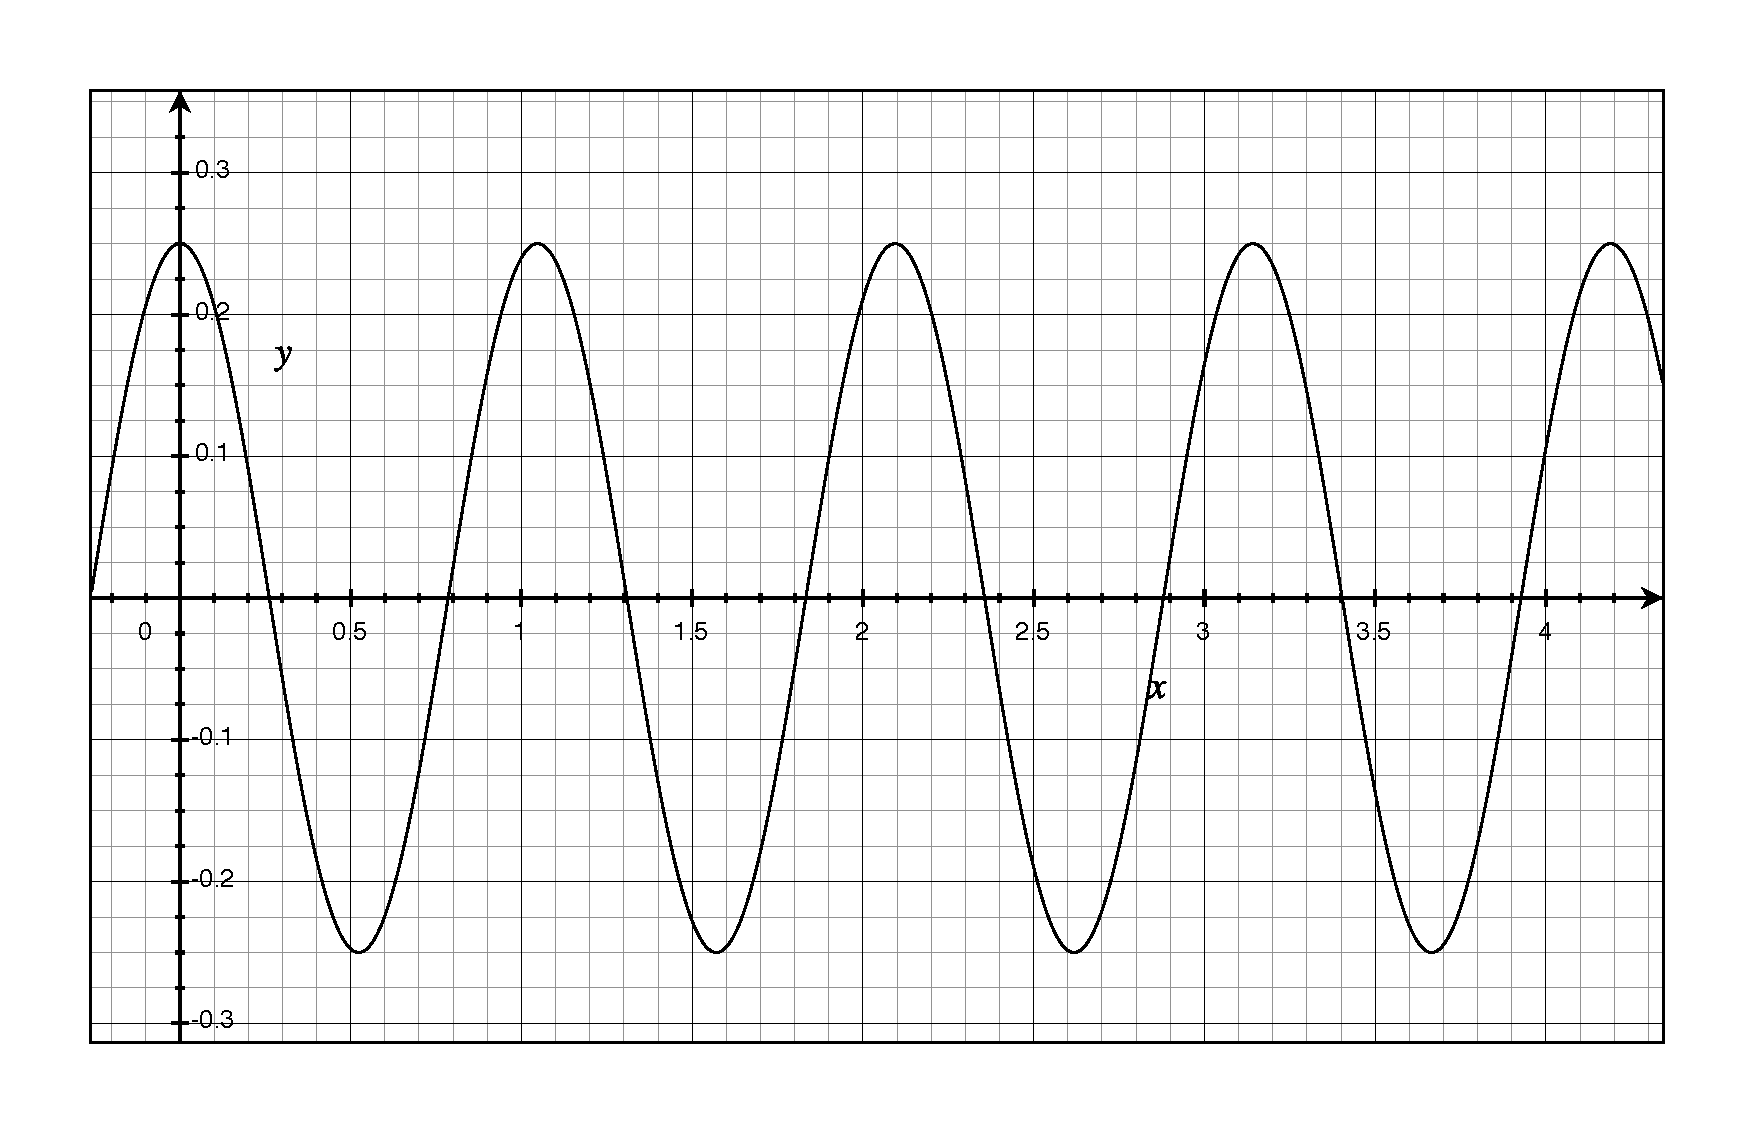
\includegraphics[scale=.3]{question59.eps}
  \caption*{Graph of Question 59}
\end{figure}

\item[60]
\begin{tabular}{ccc}
\toprule
0 & .25 & .5 \\
\midrule
.25 & 0.0138 & -0.1501 \\
\bottomrule
\end{tabular}

\begin{figure}[H]
  \centering
  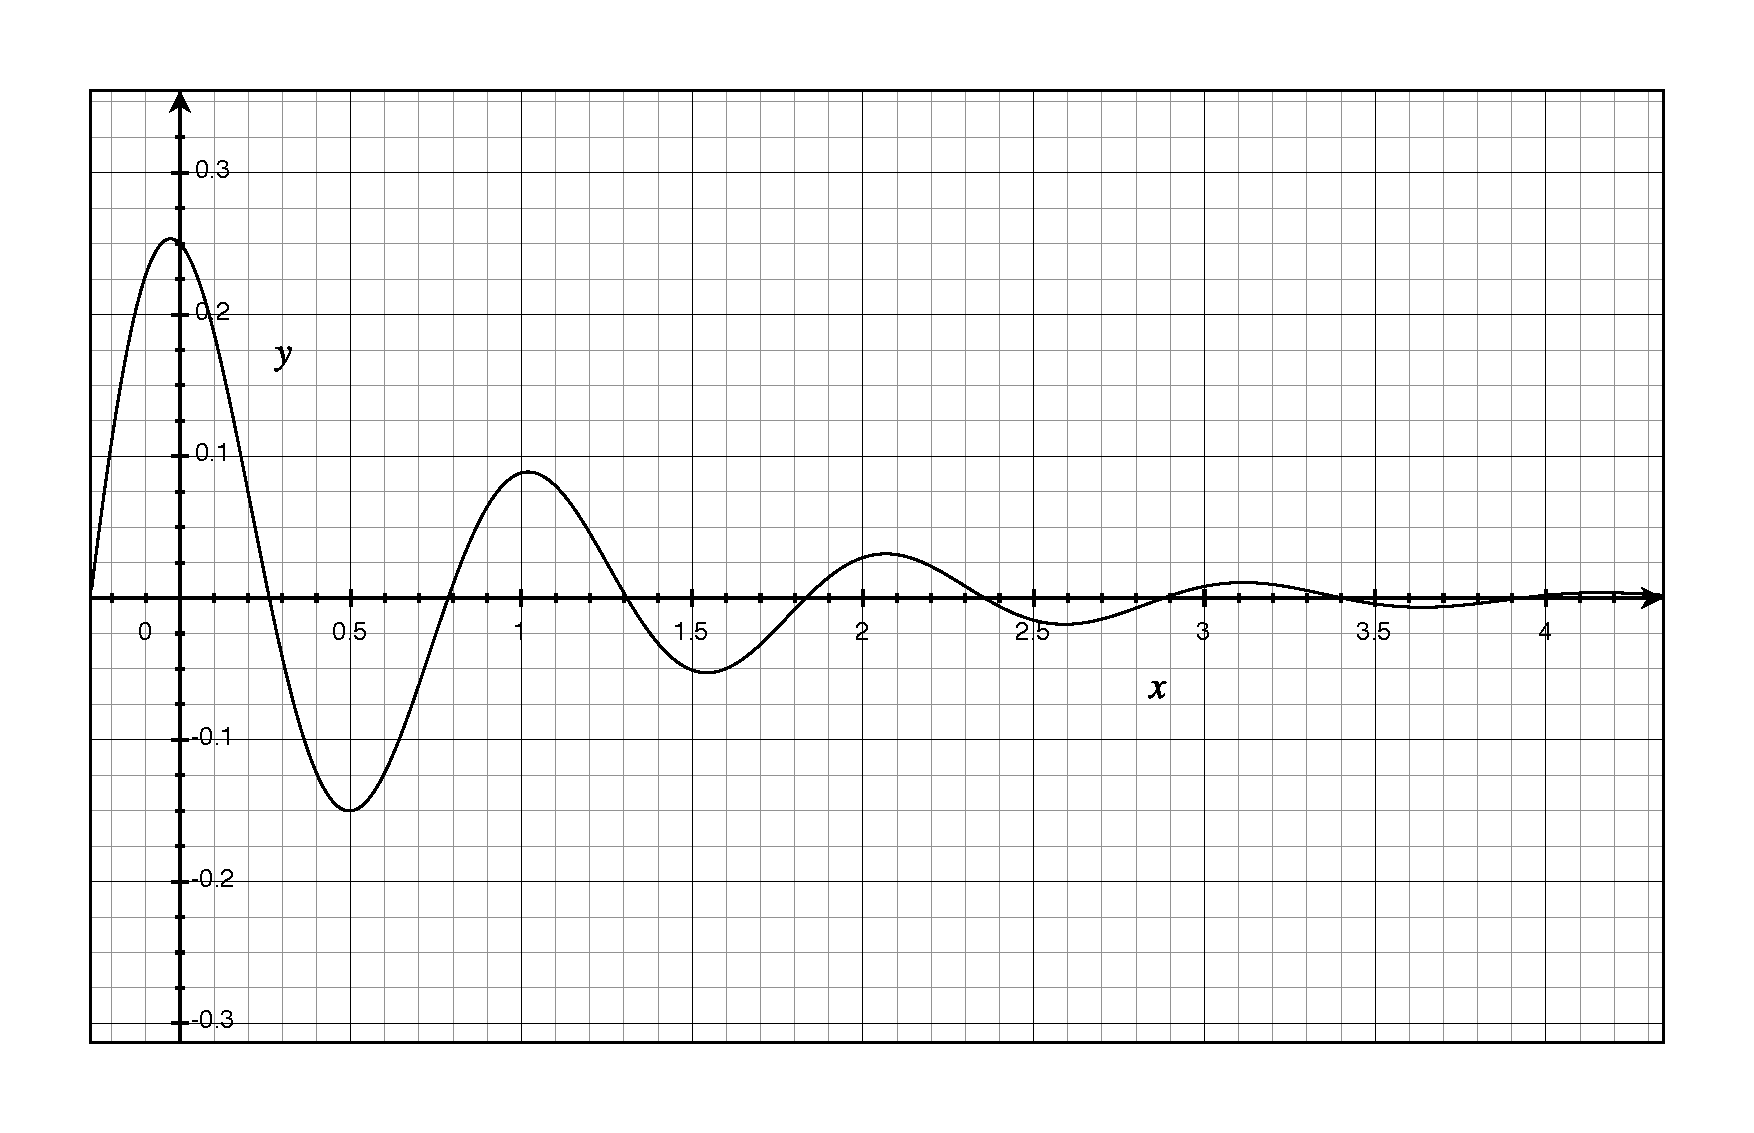
\includegraphics[scale=.3]{question60.eps}
  \caption*{Graph of Question 60}
\end{figure}

\item[61]
false.  $\sin \left( - \dfrac{3 \pi}{2} \right) = \sin \dfrac{\pi}{2} = 1$, for example

\item[62]
true.  adding any multiple of $2 \pi$ gives the same result

\end{description}

\else

\vspace{3 in}

\begin{em}
\begin{verse}
Reflected \\
in the dragonfly's eye -- \\
mountains.
\end{verse}
\end{em}
% \vspace{.1 cm}
\hspace{1.5 cm} --Issa

\fi

\end{document}

